%\documentclass[aspectratio=43]{beamer}
\documentclass[t]{beamer}
\usetheme{ffmodern}  %% Themenwahl

\usepackage[ngerman]{babel} 
\usepackage[T1]{fontenc}    % richtige Silbentrennung
\usepackage[utf8]{inputenc} % Umlaute etc.!
\usepackage{eurosym}
\usepackage{tikz}
\usepackage{pgffor}

\usetikzlibrary{arrows,decorations.pathmorphing,backgrounds,fit,positioning,shapes.symbols,chains}

%-----------------
\title{Freifunk Hamburg}
\author{In Hamburg funkt man frei\newline\newline\newline\newline\newline\newline\newline\newline @kantorkel}
\date{18. Dezember 2015}
\license{CC-BY-3.0}

\begin{document}
  \maketitle
  
  %-----------------  
  \begin{frame}{Was ist freifunk?}
    \begin{itemize}
      \item Initiative für freie, offene, kostenlose Netzwerke
      \item Steht jedem offen, als Nutzer oder Anbieter
      \item Netz in Nutzerhand
      \item Nicht kommerziell
      \item Nutzt freie, quelloffene Programme
      \item Netzneutral
    \end{itemize}
  \end{frame}
  
  %-----------------
  \begin{frame}{Verbreitung}
    \begin{columns}
      \begin{column}{0.6\textwidth}
	\begin{itemize}
	  \item In  \href{http://freifunk.net/wie-mache-ich-mit/community-finden/}{246 Orten} gibt es bereits Freifunknetze mit mehr als 26.900 Zugangspunkten
	  \item Kooperation mit Stadtverwaltungen
	\end{itemize}
      \end{column}
      \begin{column}{0.4\textwidth}
	\begin{center}
	  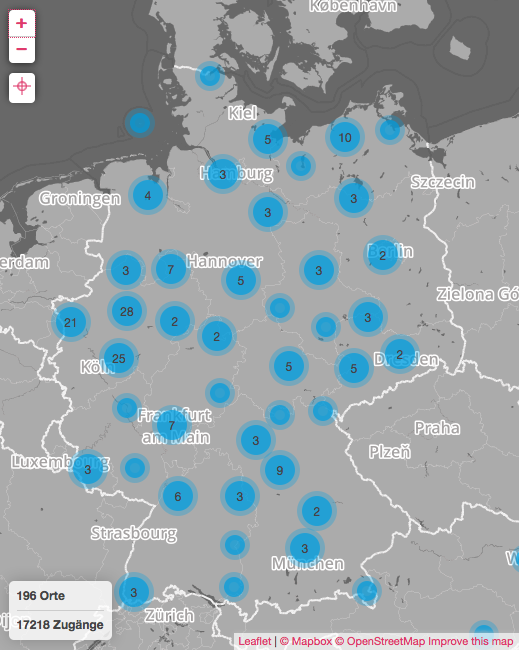
\includegraphics[width=\textwidth]{Bilder/community-map-2015-08-13}
	\end{center}
      \end{column}
    \end{columns}
  \end{frame}
  
  %-----------------
  \begin{frame}{Knotenkarte}
    \begin{center}
      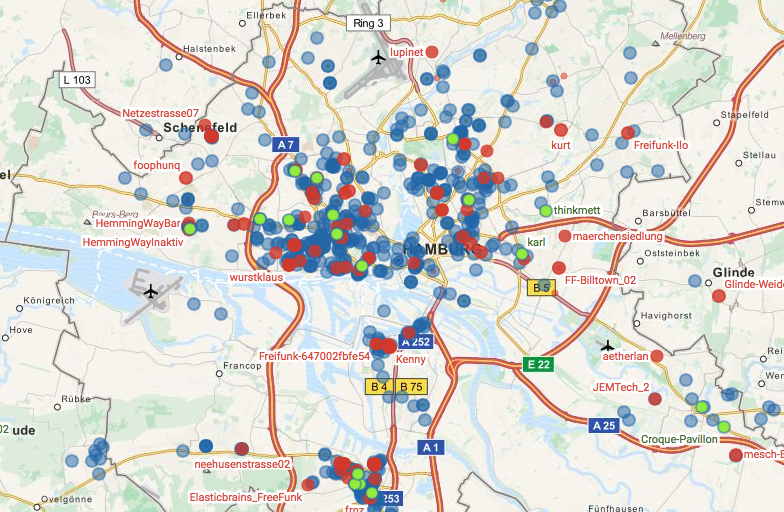
\includegraphics[width=.8\textwidth]{Bilder/knotenkarte-2015-08-13}
      \newline\tiny{Leaflet | Tiles © MapQuest, Data CC-BY-SA OpenStreetMap}
    \end{center}
    Mehr als 900 Knoten in Hamburg
  \end{frame}
  
  %----------------- 
  \begin{frame}{Freifunkknoten}
    \begin{center}
      \includegraphics[width=.6\textwidth]{Bilder/841}
    \end{center}
  \end{frame}
  \foreach \index in {1, ..., 4} 
  {
    \begin{frame}{Das Netzwerk}
      \centering \includesvg[width=9cm]{netz-\index}
    \end{frame}
  }
  
  %-----------------
  \begin{frame}{Störerhaftung}
    \begin{itemize}
      \item Keine Haftung für Knotenbetreiber
      \item Internetverkehr geht über unsere Gateways. Haftungsbefreiung nach TMG\S8.
      \item Wir nehmen die gesetzlichen Vorschriften wörtlich: Wir sammeln keine Daten.
    \end{itemize}
  \end{frame}
  
  %-----------------
  \begin{frame}{\href{http://wiki.freifunk.net/Freifunk_Hamburg/Richtfunknetz}{Richtfunknetz}}
    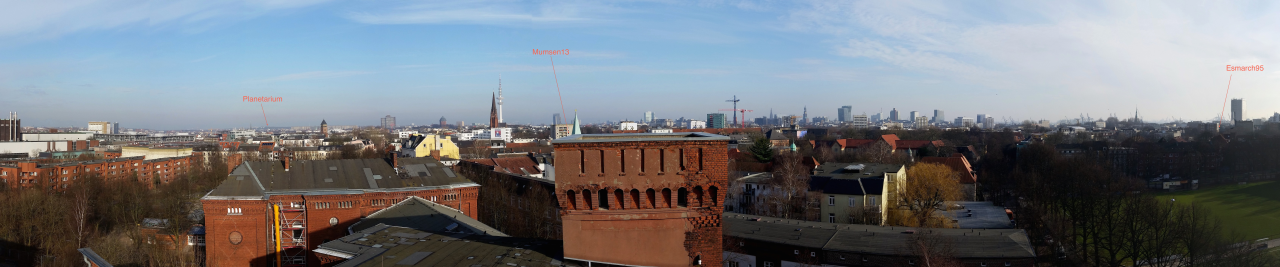
\includegraphics[width=\textwidth]{Bilder/fux}
    \begin{columns}
      \begin{column}{0.7\textwidth}
	\begin{itemize}
	  \item Eigene Infrastruktur
	  \begin{itemize}
	    \item Redundanz und Lastverteilung 
	    \item Unabhängig vom Internet
	  \end{itemize}
	\end{itemize}
      \end{column}
      \begin{column}{0.3\textwidth}
	\begin{center}
	  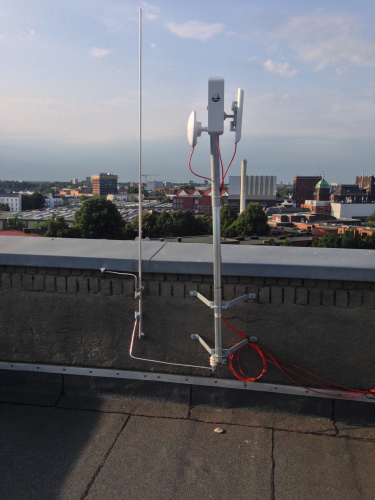
\includegraphics[width=.9\textwidth]{Bilder/richtfunkmast}
	\end{center}
      \end{column}
    \end{columns}
  \end{frame}
  
  %-----------------
  \begin{frame}{Richtfunknetz}
    \begin{center}
      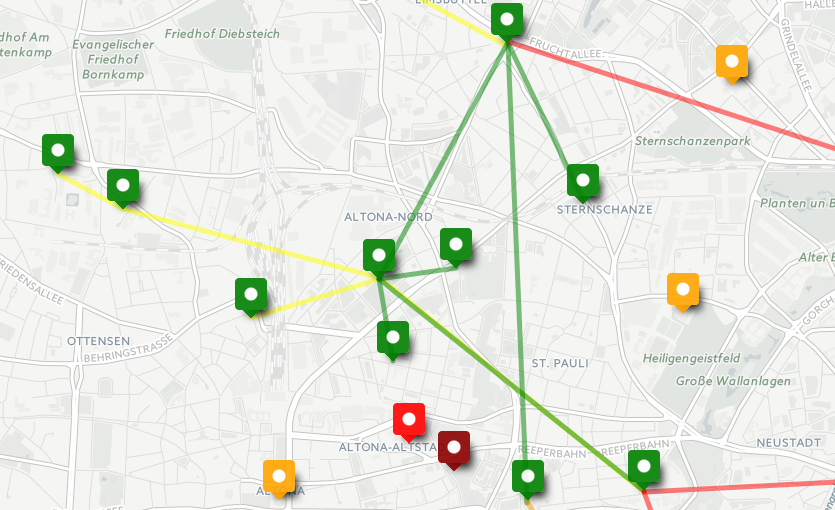
\includegraphics[width=0.95\textwidth]{Bilder/richtfunk-uebersicht}
    \end{center}
    \tiny{OSM - Deutschland Karte hergestellt aus OpenStreetMap-Daten | Lizenz: Open Database License (ODbL) | Courtesy of OpenStreetMap.de}
  \end{frame}
  
  %-----------------
  \begin{frame}{Freifunk für Flüchtlinge}
    \begin{itemize}
      \item Kommunikation ist wichtig
      \item Viele Flüchtlinge besitzen Smartphones
      \item Stadt sieht WLAN nicht als Teil der Grundversorgung
    \end{itemize}
  \end{frame}
  
  %-----------------
  \begin{frame}{2013: Embassy of Hope}
    \begin{center}
      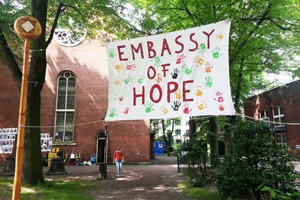
\includegraphics[width=.4\textwidth]{Bilder/embassyofhope.jpg} 
    \end{center}
    \begin{itemize}
      \item 300 Flüchtlinge aus Libyen sind in der St. Pauli Kirche untergekommen
      \item Router vorfinanziert und an einem Wochenende aufgebaut
      \item Geld hinterher binnen weniger Stunden eingesammelt
    \end{itemize}
  \end{frame}
  
  %-----------------
  \begin{frame}{2014: Schwarzenbergplatz}
    \begin{center}
      
\includegraphics[width=.8\textwidth]{Bilder/schwarzenberg}
    \end{center}
    \begin{itemize}
      \item Containerdorf für zunächst 250 Menschen
      \item Ich wohne gegenüber: Uplink!
      \item Inzwischen mehr als 700 Menschen
    \end{itemize}
  \end{frame}
  
  %-----------------
  \begin{frame}{2014: Schwarzenbergplatz}
    \begin{center}
      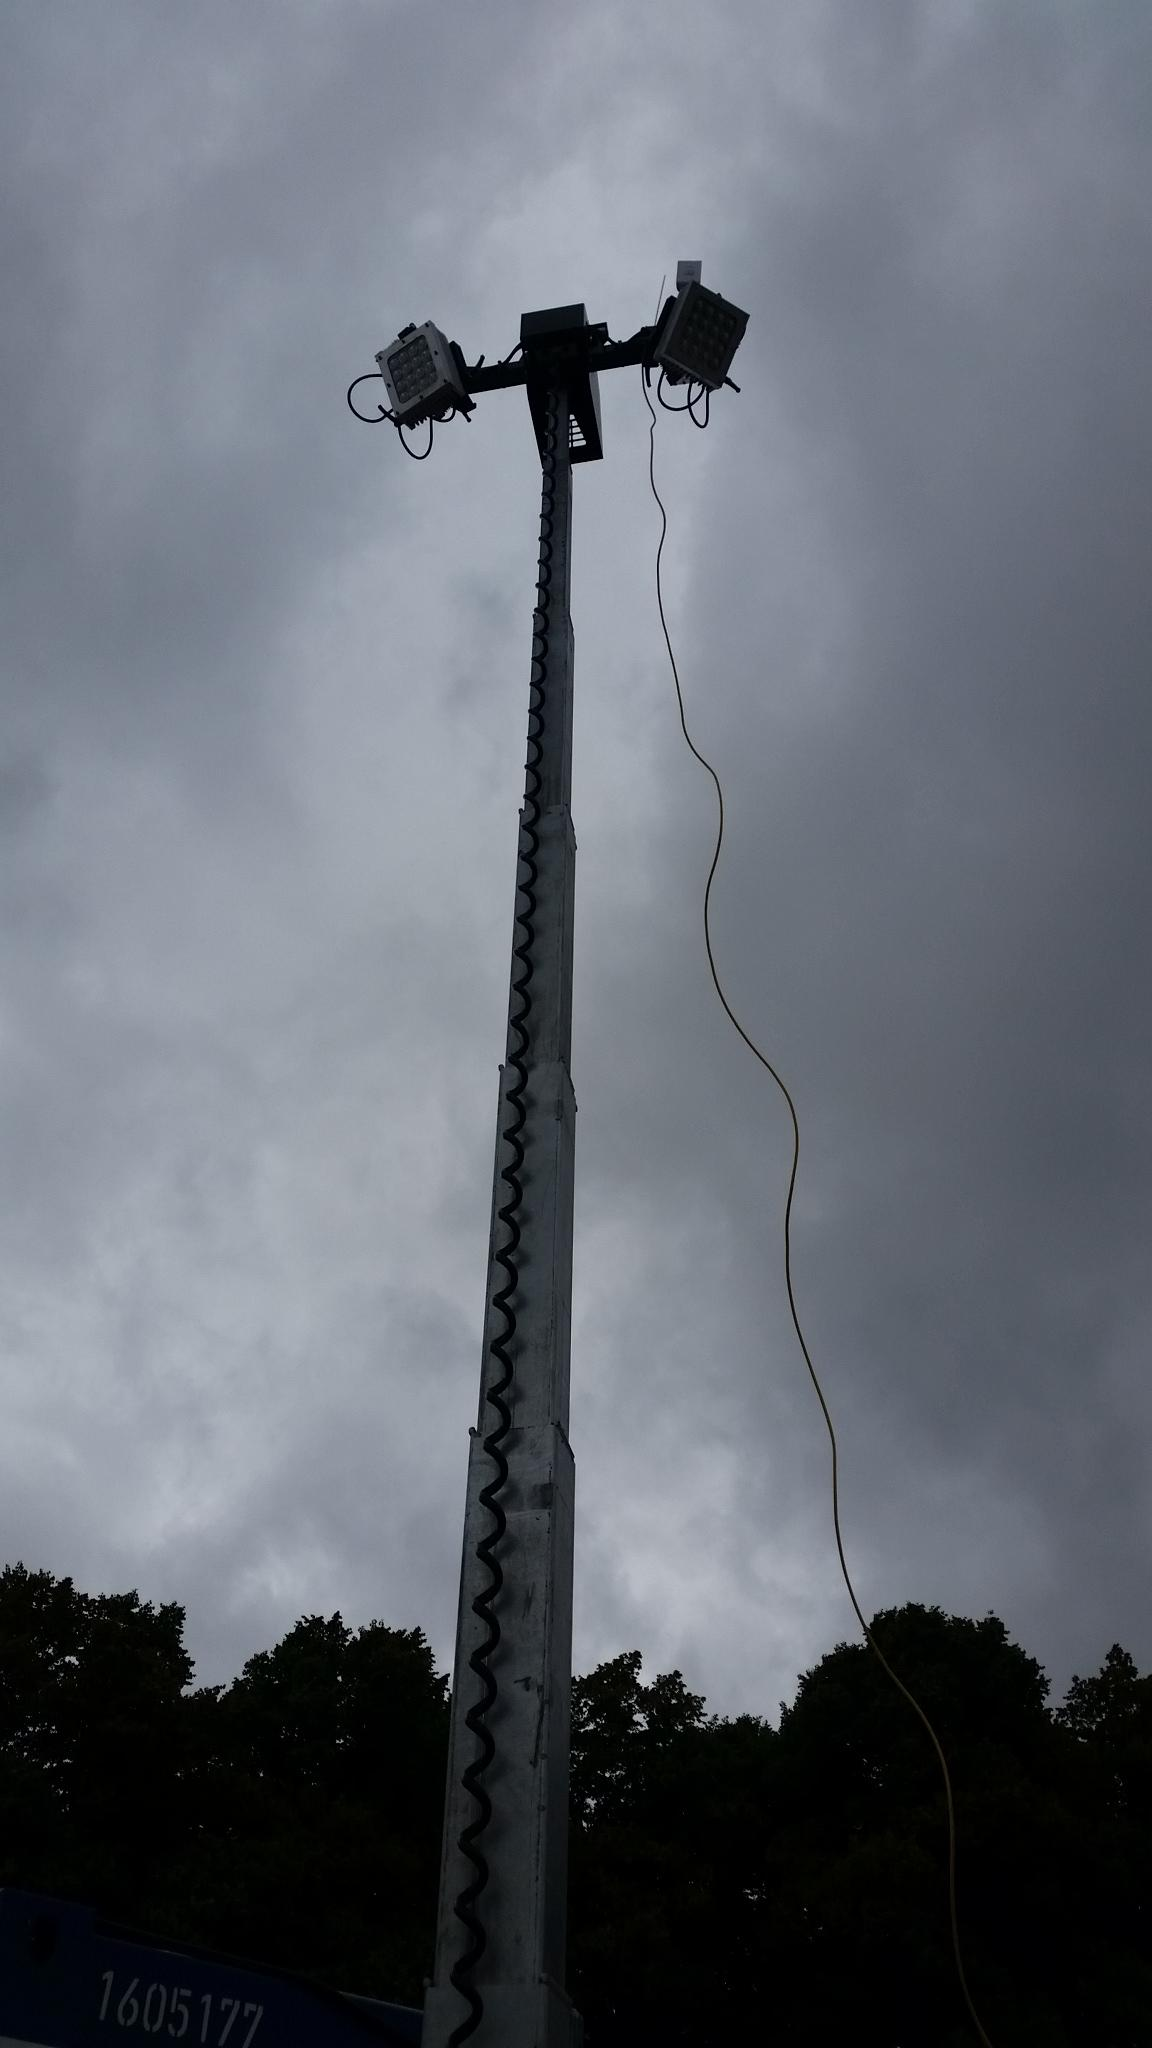
\includegraphics[width=.4\textwidth]{Bilder/schwarzenberg-lichtmast}
    \end{center}
  \end{frame}
  
  %-----------------
  \begin{frame}{2014: Schwarzenbergplatz}
    \begin{center}
      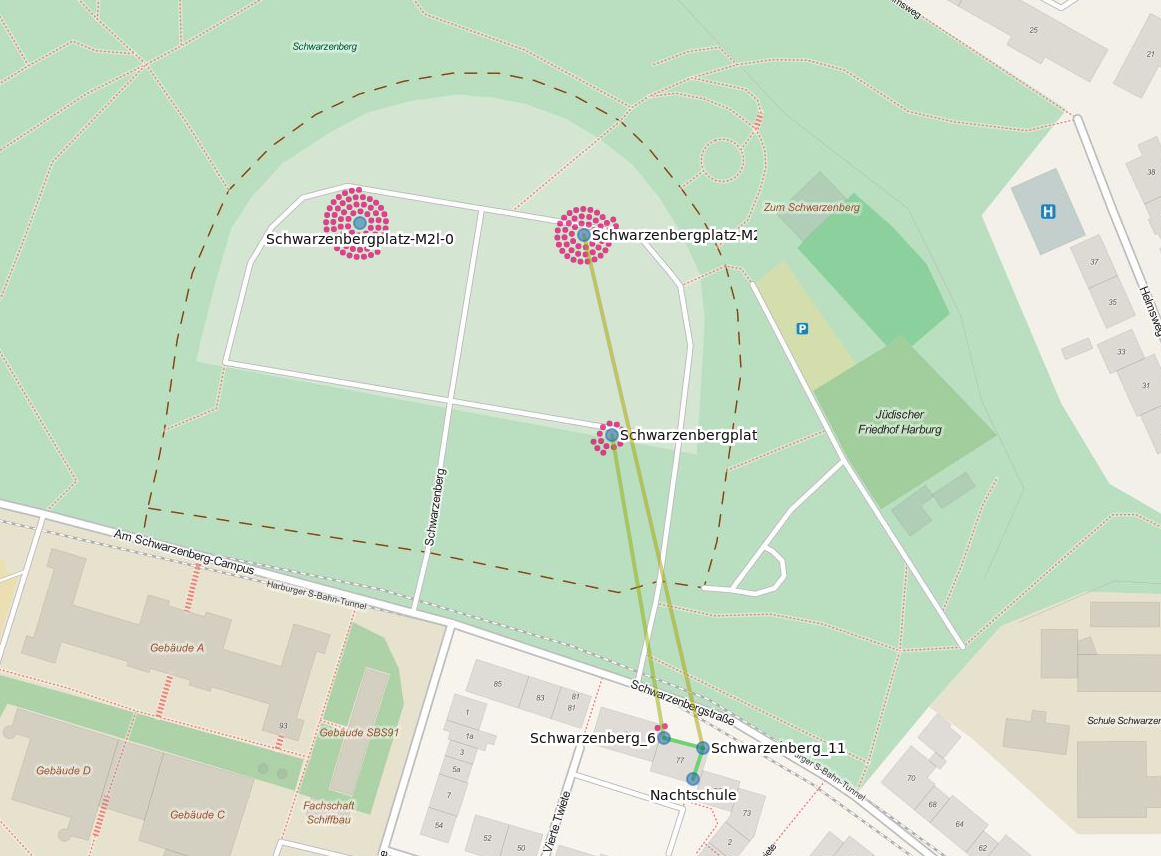
\includegraphics[width=.7\textwidth]{Bilder/schwarzenberg-2015-09-22}
      \newline\tiny{Leaflet | Tiles © MapQuest, Data CC-BY-SA OpenStreetMap}
    \end{center}
  \end{frame}
  
  %-----------------
  \begin{frame}{2015}
    \begin{itemize}
      \item Flüchtlingsschiff Transit, Messehallen, Hauptbahnhof, u.a.
      \item Und ca. 15 weitere Standorte, an denen Menschen freifunken wollen!
      \item Howto?
    \end{itemize}
  \end{frame}
  
  %-----------------
  \begin{frame}{Howto?}
    \begin{itemize}
      \item Uplink finden
      \item Hardwarebedarf schätzen
      \item Geräte finanzieren und aufstellen
      \item Dokumentieren
      \bigskip
      \item \small{ \href{https://wiki.freifunk.net/Hamburg/Flüchtlinge}{https://wiki.freifunk.net/Hamburg/Flüchtlinge}}
    \end{itemize}
  \end{frame}
  
  %-----------------
  \begin{frame}{Freifunk lebt vom Mitmachen}
    \begin{itemize}
      \item Wir sind kein Dienstleister
      \item aber wir geben unser Wissen gerne weiter
    \end{itemize}
  \end{frame}
  
  %-----------------
  \begin{frame}{Wie kann ich mitmachen?}
    \begin{itemize}
      \item Router aufstellen
      \item Freifunk Treffen
      \begin{itemize}
       \item Montags, 19 Uhr, CCCHH, Zeiseweg 9
       \item Freitags, 19:30 Uhr, Attraktor, Eschelsweg 4
      \end{itemize}
      \item Mailingliste
      \begin{itemize}
       \item \href{mailto:freifunk@hamburg.ccc.de}{freifunk@hamburg.ccc.de}
      \end{itemize}
      \item IRC
      \begin{itemize}
       \item \#ffhh auf hackint.org
      \end{itemize}
      \item Wiki, Pads, Forum, \ldots
    \end{itemize}
  \end{frame}
  
  %-----------------
  \begin{frame}{Vielen Dank!}
    \begin{center}
      \includesvg[width=3.5cm]{in-hamburg-funkt-man-frei}
    \end{center}
    \begin{itemize}
      \item Netz: \href{https://hamburg.freifunk.net}{https://hamburg.freifunk.net}
      \item Mail: \href{mailto:kontakt@hamburg.freifunk.net}{kontakt@hamburg.freifunk.net}
      \item Treffen: Montags \& Freitags, \href{https://hamburg.freifunk.net/kalender}{https://hamburg.freifunk.net/kalender}
    \end{itemize}
  \end{frame}
  
\end{document}